\documentclass{replab}
\usepackage{lipsum}

% --- Información del documento ---
\title{Práctica 1}                              % Practica #
\subtitle={Titulo de la Práctica}               % Titulo
\subject={Laboratorio de Electromagnetismo}     % Materia
\date{\today}                                   % Fecha

% --- Autores ---
\author[1]{Luis Gerardo De Asís Venegas \thanks{LuisDeAsisV@ciencias.unam.mx}}
\author[1]{Zahid Medrano Flores \thanks{zahidmedrano@ciencias.unam.mx}}
\author[1]{Daniel Santiago Gallegos \thanks{daniel\_santiago07@ciencias.unam.mx}}

\affil[1]{Facultad de Ciencias, Universidad Nacional Autónoma de México, Ciudad Universitaria, Coyoacán, 04510, México, CDMX}

\setlength{\columnsep}{14pt}

% --- Archivo de bibliografía ---
\addbibresource{ref.bib}

% --- Inicio del documento ---
\begin{document}
	
    \singlespacing
	\pagestyle{fancy}
	\unspacedoperators
	
% --- Título ---
\selectlanguage{spanish}
	
% --- Cuerpo del reporte ---

\twocolumn[
    \begin{center}
        \maketitle
        \hrulefill
        \vspace{-5pt}
            \begin{onecolabstract}

                \vspace{-12pt}

                El resumen se redacta en pasado simple, en impersonal y modo indicativo (p.e. se realizó un...); en la medida de lo posible se debe evitar los pasados imperfectos y tiempos compuestos (p.e. se estaba realizando un...o se ha venido realizando un...). Usualmente el resumen contiene una breve introducción con relación al tema de la práctica (una o dos líneas), posteriormente una breve explicación del trabajo realizado, así como la metodología usada (de tres a cuatro líneas) y finalmente un bosquejo de los resultados más relevantes de la práctica (de dos a cuatro líneas). Debe ante todo cumplir con la respuesta a las preguntas importantes del desarrollo del problema: ¿Que se hizo? ¿Como se hizo? ¿Dónde se hizo? ¿Cuándo se hizo? ¿Que consiguió? ¿Que recomienda?

                \medskip

                \noindent\textit{Palabras clave:} algunas, palabras, importantes, relacionadas, con, el, experimento.
            \end{onecolabstract}

        \vspace{-10pt}

            \selectlanguage{english}
            \begin{onecolabstract}

                \vspace{-12pt}
                
                The summary is written in the simple past, in the impersonal and indicative mood...

                \medskip

                \noindent\textit{Keywords:} some, important, words, related, to, the, experiment.
                \end{onecolabstract}
        \hrulefill
        \vspace{-5pt}
    \end{center}
]

\bigskip
	
% --- Cuerpo del reporte ---

\bigskip
\saythanks
	
\section{Introducción}

Contiene una breve reseña asociada al tema de la práctica, (de dos a cuatro líneas), así como las definiciones y conceptos relevantes de la práctica. Además, contiene las ecuaciones a utilizar en el desarrollo de la práctica (las ecuaciones podrían también presentarse en la sección de desarrollo experimental). Los conceptos y definiciones relacionados a la práctica deben ser redactados adecuadamente. Es decir, el orden en que se presenten las ideas debe ser el adecuado para la compresión y claridad del manuscrito. Además, las ideas deben ser claras, concretas y completas. Se deben evitar faltas de ortografía como, por ejemplo, palabras mal escritas o que no se presenten adecuadamente los diferentes signos de puntuación.

El texto no debe copiarse textualmente de las fuentes consultadas, se deben parafrasear las ideas y citar la referencia de donde se está consultando la información. Las referencias deben estar citadas en el texto, usando el número de cita de la lista contenida en la sección de referencias. Existen gestores de bibliografía como Zotero, EdNote y Mendeley que facilitan la tarea y pueden enlazarse con facilidad en Overleaf. Se recomienda que el formato de cita a utilizar sea el empleado por la comunidad científica de la IEEE (p.e. Buckley et al. [1], como ha sido demostrado [1], etc.).

Si en esta sección se incluyen las ecuaciones, estas deben aparecer en un orden lógico acorde a la secuencia en que se comiencen a presentar los conceptos y definiciones.
Las ecuaciones deberán de ir enumeradas y deberán describirse cada una de sus variables, además, si fueron extraídas de algún libro o artículo se deberá de colocar la referencia correspondiente antes de mostrar la ecuación. Como se muestra a continuación:
“La elasticidad es la capacidad de los materiales de recuperar su tamaño y su forma cuando se quitan las fuerzas que les producen deformaciones. Esta propiedad se encuentra en mayor o menor medida en todos los cuerpos sólidos \cite{hecht}:

\begin{equation}
    \epsilon = \frac{\Delta L}{L} = \frac{F}{AE}
\end{equation}

Siendo $\Delta L$ el alargamiento, $L$ la longitud original, $E$: módulo de Young, $A$ la sección transversal de la pieza estirada. La ley se aplica a un cuerpo elástico hasta un límite denominado límite elástico. La forma más común de representar matemáticamente la Ley de Hooke es mediante la ecuación del muelle o resorte, donde se relaciona la fuerza $F$ ejercida por el resorte con la elongación o alargamiento $\delta$ provocado por la fuerza externa aplicada al extremo de este \cite{feynman}:

\begin{equation}
    F = -k \delta
\end{equation}

Donde $k$ se llama constante elástica del resorte y $\delta$ es su elongación o variación que experimenta su longitud.”

Además, el formato de los diferentes símbolos empleados para definir las operaciones debe ser el adecuado, así como presentar en cursiva solo aquellas variables que puedan tener diferentes valores (las constantes se presentan sin cursiva). Adecuada presentación de las variables vectoriales.

Finalmente, cabe mencionar que las ecuaciones deben estar citadas en el texto, definiendo las variables asociadas a cada expresión matemática sin asignar la misma letra a dos o más variables de distinta naturaleza y con esto causar confusión o poca claridad en la comprensión del reporte. Además, las variables deben tener el mismo formato de letra en el texto y en las ecuaciones.

\section{Objetivo general}

Mencionar en forma general cual es el propósito de la práctica y como se alcanzará este propósito en forma breve.

\section{Objetivos particulares}

Mencionar la forma en que se alcanzará el objetivo general mediante objetivos más específicos, esto mediante los experimentos que se realizarán en la práctica.

\section{Hipótesis}

La hipótesis es una conjetura formulada en base a la percepción, intuición, experiencia e información conocida sobre algún tema particular. Esta deberá de confirmarse o desecharse a partir de los resultados obtenidos en la práctica.

\section{Equipo y material}

En esta sección sólo debe de contener el equipo y material realmente fue usado en la práctica. Con sus correspondientes características técnicas.

\section{Desarrollo Experimental}

En esta sección se debe describir la metodología y el procedimiento de forma detalla, es decir, cómo se llevaron a cabo los experimentos especificando el material y el equipo usado, así como el montaje experimental (se deberán agregar las figuras). La información debe ser suficiente para que el trabajo sea reproducible. Si en esta sección se incluyen las ecuaciones de la práctica (para deducir nuevos datos a partir de los hallados en los experimentos), estas deben aparecer en un orden lógico acorde a la secuencia en que se fueron realizando los experimentos y se fueron obteniendo los resultados. Si las ecuaciones fueron presentadas en la introducción, ellas no deben volver a presentarse en la sección de desarrollo experimental, basta con citarlas acorde al número de ecuación.

Las figuras deben estar con número y con su descripción correspondiente. Esta información debe colocarse en la parte inferior de la figura (Ver figura \ref{fig:numerouno}). Las letras y números de las figuras deben ser consistentes con el formato usado en el manuscrito. La información mostrada en las figuras debe ser legible, es decir, las letras o números contenidos en la figura deben tener el suficiente tamaño y no deben verse borrosas. Las figuras deben estar citadas en el texto antes de ser presentadas en el manuscrito. Finalmente, en las gráficas se deben definir los ejes con sus correspondientes unidades, en la descripción de la figura se deben de explicar el significado de puntos, curvas o algún otro elemento relevante de la gráfica.

\begin{figure}[hbt!]
    \centering
    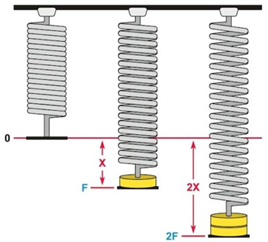
\includegraphics[width=0.7\columnwidth]{imágenes/Imagen1.png}
    \caption{Experimento del número de Reynolds.}
    \label{fig:numerouno}
\end{figure}

\section{Resultados y discusión}

\textit{Resultados}. Esta sección contiene los resultados derivados de la práctica mediante tablas y figuras (como podrían ser gráficas). Esta sección podría contener ecuaciones, por ejemplo, en las prácticas donde se tengan que realizar ajustes para describir el comportamiento de los datos obtenidos experimentalmente, la ecuación obtenida a partir del ajuste es un resultado más. Finalmente, no deben ser colocadas de forma textual las operaciones realizadas para obtener nuevos datos, ya que, se entiende que este proceso se realiza por medio de hojas de cálculo, es suficiente que en esta sección se presenten todos los datos obtenidos experimentalmente y los derivados de las ecuaciones (en forma de tablas y gráficas), en principio no debería haber confusión de cómo es que se obtuvieron esos resultados o datos porque esto ya fue explicado en la sección de desarrollo experimental. Los resultados deben ser acompañados con el texto necesario para guiar al lector en la comprensión y entendimiento de la información presentada.

Las tablas deben presentarse como Tabla 1, Tabla 2, etc., además deben estar con número y con su descripción correspondiente. Esta información debe colocarse en la parte superior de la tabla. Las letras y números de las tablas deben ser consistentes con el formato usado en el manuscrito. La información mostrada en las tablas debe ser legible, es decir, las letras o números contenidos en la tabla deben tener el suficiente tamaño y no deben verse borrosas. Las tablas deben estar citadas en el texto antes de ser presentadas en el manuscrito.

El formato de las tablas deberá de ser el siguiente:

\begin{table}[hbt!]
    \centering
    \footnotesize
    \caption{Ejemplo de un cuadro con propiedades}
    \label{tab:propiedades}
    \begin{tabularx}{\columnwidth}{lYY}
            \hline
            \textbf{Compuesto} & \textbf{$M$/(g/mol)} & \textbf{$T_{eb}^{\circ}$/(°C)} \\
            \hline
            $H_2O$      & 18.02     & 100   \\
            $CO_2$      & 44.01     & -     \\
            $H_2SO_4$   & 98.079    & 337   \\
            \hline
    \end{tabularx}
\end{table}

\textit{Análisis}. Contiene una correcta interpretación de los resultados. Las afirmaciones y conclusiones que se deriven de la práctica deben fundamentarse en los resultados obtenidos.

\section{Conclusiones}

Esta sección contiene afirmaciones obtenidas a partir de las observaciones experimentales. Así cada afirmación o idea presentada en esta sección debe de estar basada o respaldada en los resultados obtenidos en la práctica.

Se expresa concretamente la aceptación o el rechazo de las hipótesis planteadas al inicio del estudio y cómo se lograron los objetivos planteados en la investigación.

Asimismo, de acuerdo con la discusión se indican los hechos y deducciones relevantes. Es necesario señalar los errores y/o limitaciones observadas en la metodología empleada.

\section{Observaciones}

Es necesario señalar los errores y/o limitaciones observadas en la metodología empleada.

\section{Recomendaciones}

En función de los errores y/o limitaciones observadas proponer recomendaciones para mejorar los métodos utilizados.

\section*{Nomenclatura}

Los símbolos usados para las abreviaturas de las unidades de las cantidades físicas deben ser consistentes en todo el texto.

\vspace{1em}

\begin{tabular}{ll}
  $\mu$      & Viscosidad, kg/(ms) \\
  $\rho$     & Densidad, kg/m$^3$ \\
  $D$        & Diámetro, m \\
  $N_{Re}$   & Número de Reynolds, adim. \\
  $V$        & Velocidad, m/s \\
\end{tabular}

\printbibliography[heading=bibintoc]

{
\appendix
\section{}

Para el cálculo de la densidad se empleó la siguiente ecuación:

\begin{equation}
    \rho = \frac{m_{total} - m_{probeta}}{V_{muestra}}
\end{equation}

\section{}

B

}

\end{document}